\documentclass[a4paper,11pt]{article}
\usepackage[latin1]{inputenc}
\usepackage[T1]{fontenc}
\usepackage{amsmath}
\usepackage{a4wide}
\usepackage{url}
\usepackage{booktabs}
%\usepackage{enumitem} % to remove lists indent with \begin{itemize}[leftmargin=*]
\usepackage{graphicx}
\usepackage{wrapfig}


\title{Genomics and Bioinformatics}
\date{November 1, 2011}
\author{Examination - Week 7}
\begin{document}


\section*{Question 3}


\setlength\intextsep{0pt}
\begin{wrapfigure}{r}[-15pt]{0.20\textwidth}
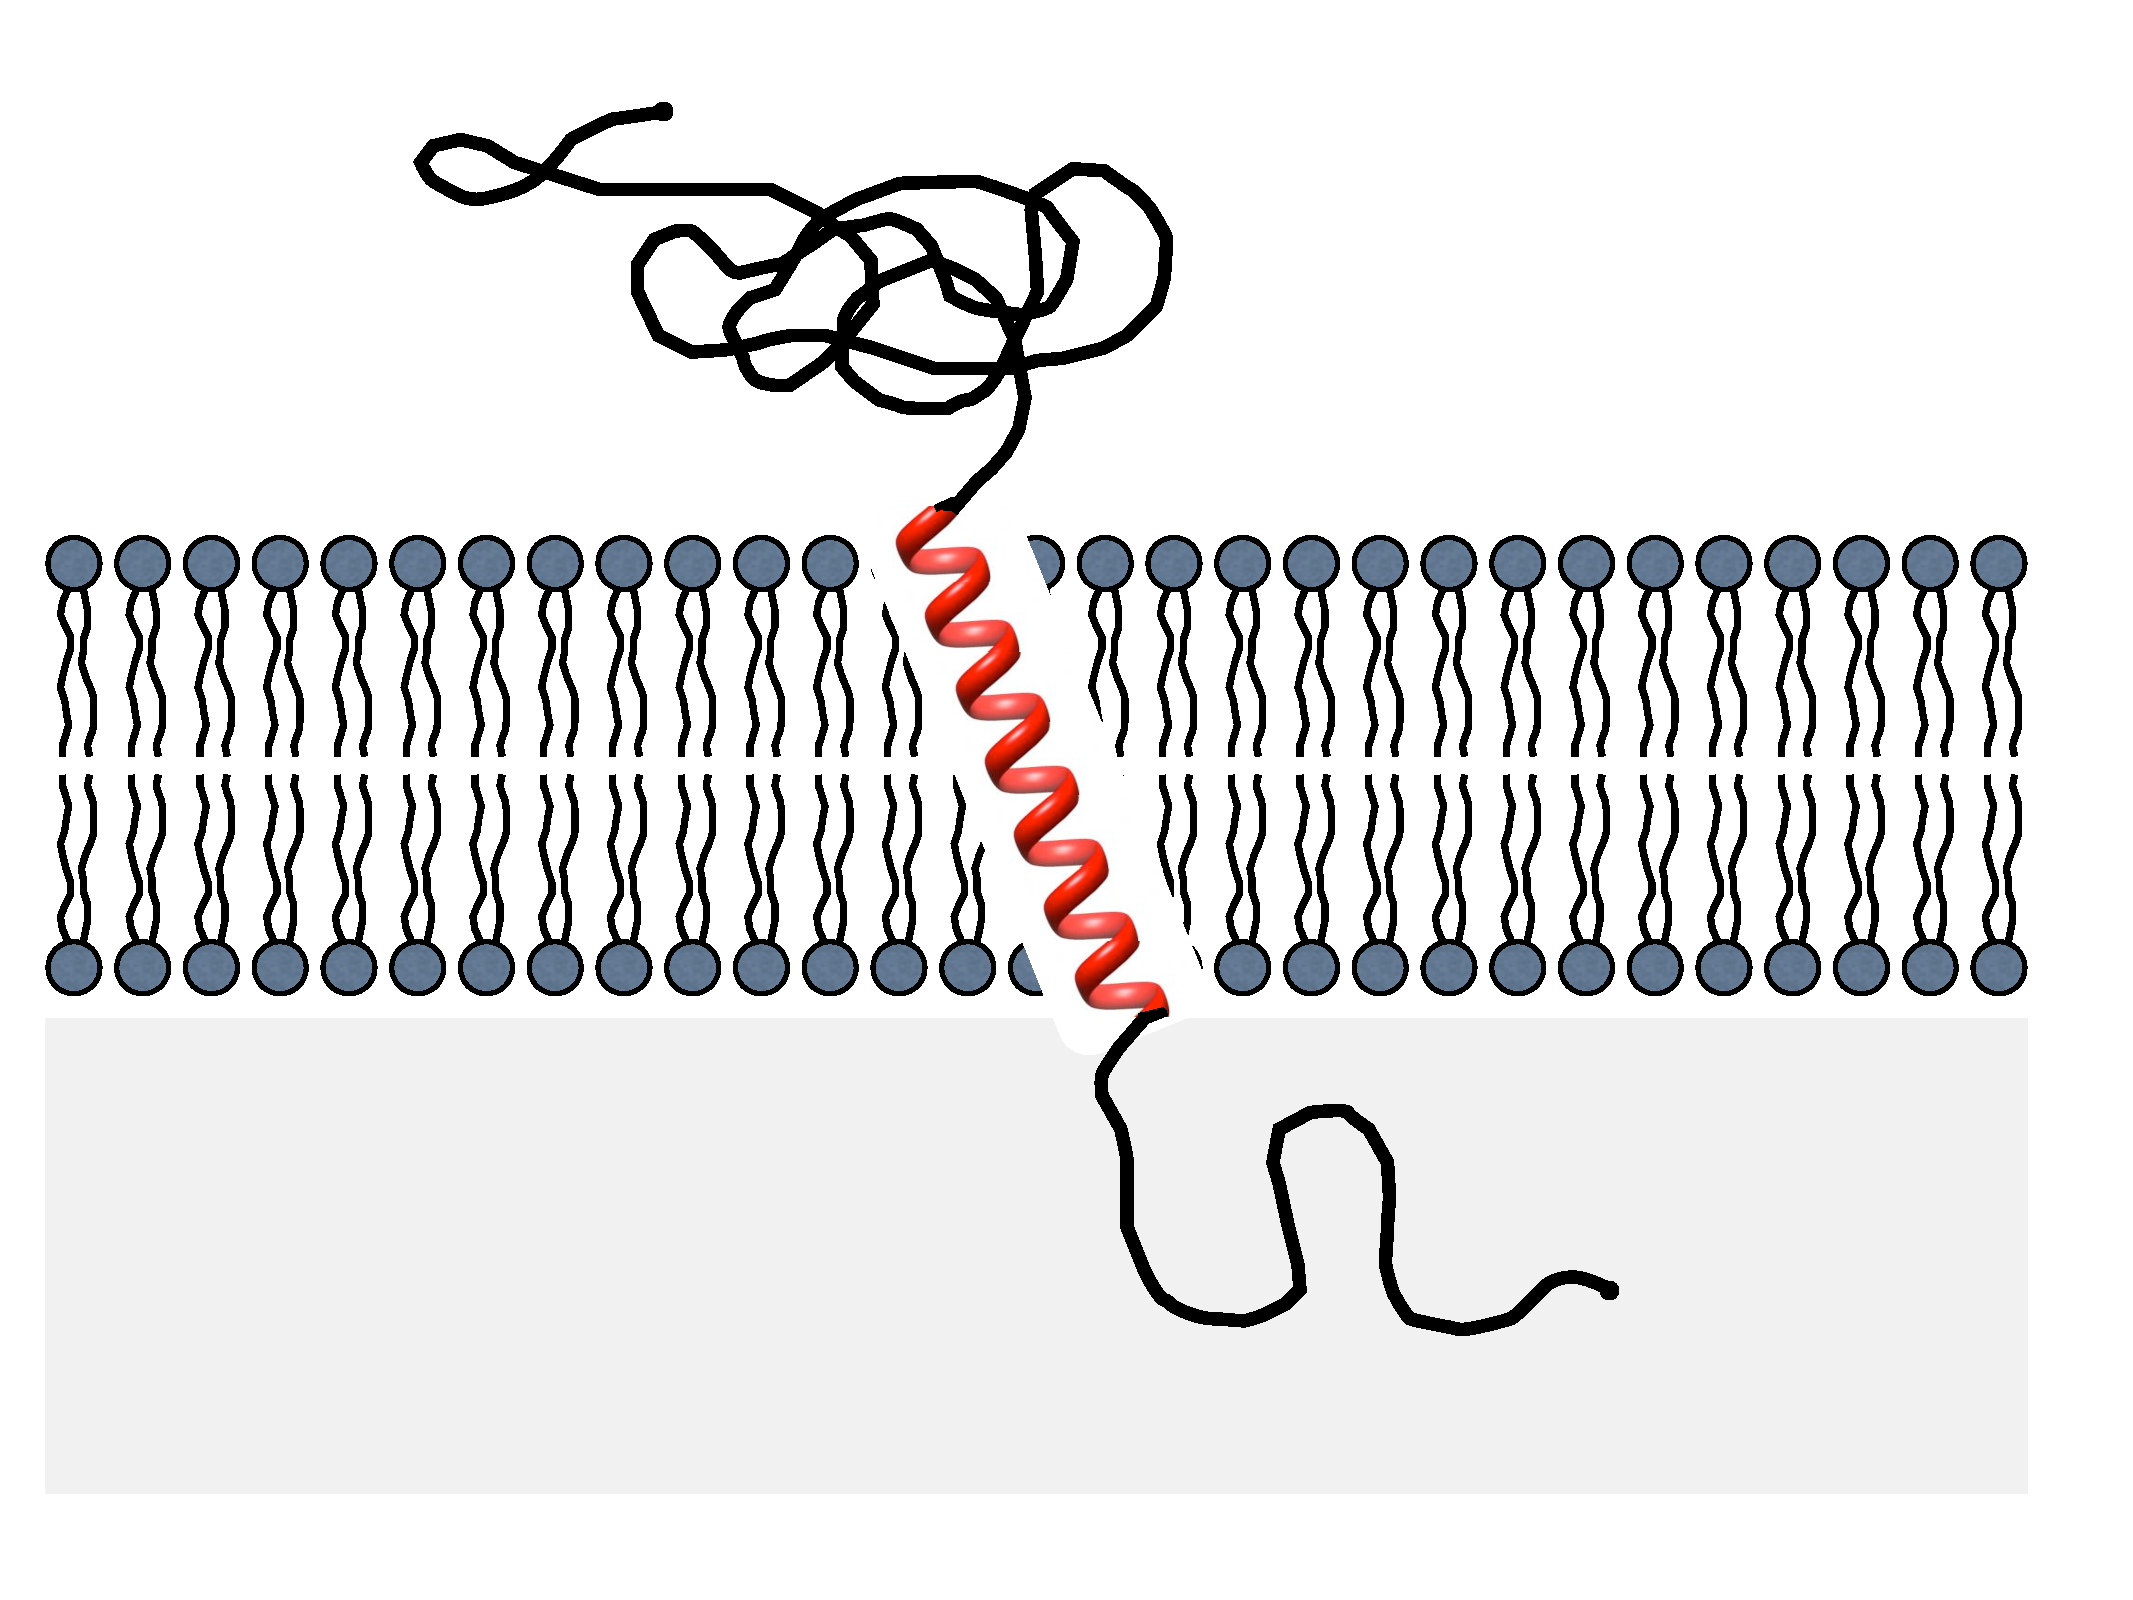
\includegraphics[width=0.3\textwidth]{figures/transmembrane.pdf}
\end{wrapfigure}

A transmembrane protein is a protein that has one or more domains going from one side of the 
plasmic membrane through to the other side. As a consequence, they have extracellular, 
intracellular and transmembrane domains. 
Very often the transmembrane domains are structures 
known as ``alpha-helices''. We want to find them using a Hidden Markov Model.

The propensity of different amino-acids to be part of an alpha-helix is well-known and scored in the table below.
For this exercise we assume that:
\begin{itemize}%[leftmargin=*]
\item All transmembrane domains are alpha-helices of appropriate length: in average 20 amino-acids.
\item In other domains of a protein, amino-acids are equally distributed.
\item Intracellular domains are in average 200 amino-acids long and extracellular domains, 500.
\end{itemize}

%% From Wiki:
%\begin{table}[h]
 %\caption{Helical propensity of amino-acids: difference in free energy relative to Alanine arbitrarily set to zero.}
 % \begin{center}
  %  \begin{tabular}{ cccccccccc c }
   %   A & R & N & D & C & E & Q & G & H & I \\
    %  0 & 0.2 & 0.7 & 0.7 & 0.7 & 0.4 & 0.4 & 1 & 0.6 & 0.4 \\
    %\\
    %  L & K & M & F & P & S & T & W & Y & V \\
    %  0.2 & 0.3 & 0.2 & 0.5 & 3.2 & 0.5 & 0.7 & 0.5 & 0.5 & 0.6 \\
   % \end{tabular}
 % \end{center}
%\end{table}

\begin{table}[h]
 \caption{Helical propensity of amino-acids, as the fraction of each type found in helices.}
  \begin{center}
    \begin{tabular}{ cccccccccc c }
      A & R & N & D & C & E & Q & G & H & I \\
      \bf{8\%} & 7\% & 4\% & 4\% & 4\% & 6\% & 6\% & 3\% & 5\% & 6\% \\
    \\
      L & K & M & F & P & S & T & W & Y & V \\
      7\% & 6\% & 7\% & 5\% & \bf{0.3\%} & 5\% & 4\% & 5\% & 5\% & 5\% \\
    \end{tabular}
  \end{center}
\end{table}


\begin{enumerate}%[leftmargin=*]
\item Propose the structure of a simple Hidden Markov Model to predict transmembrane domains 
from a given amino-acids sequence. Draw a diagram.
\item What are the emission probabilities?
\item Based on the length of the respective domains, give an estimate of the transition probabilities. Write the transition matrix.
\item Here is the sequence of a dummy transmembrane protein.
$$\mbox{NGAKTTL}$$
How woud you calculate the probability of observing this sequence, given the model? (Do not calculate it).

\item Here is the sequence of a dummy transmembrane protein, where the transmembrane domain
is known and underlined.
$$\mbox{NG\underline{AK}TTL}$$
What is the probability of observing this sequence? 

\item \textit{Bonus:} how would you adapt the model (only the diagram) if moreover you know that an alpha-helix is defined as 
hydrogen bounds linking groups of 4 amino-acids?
\end{enumerate}

\end{document}
